% Конструкторский раздел
\chapter{Конструкторский раздел}

В данном разделе разработана структура базы данных медицинской клиники, определены ограничения целостности, процедуры, триггеры, роли и правила кэширования.

\section{Схема проектируемой базы данных}

База данных разделена на логические схемы безопасности, справочников, расписания, медицинских и финансовых данных. Такое разбиение позволяет отделить подсистему безопасности от справочных, операционных и финансовых данных. ER-диаграмма сущностей приведена в аналитическом разделе (рисунок~\ref{fig:er-diagram}).

Схема проектируемой базы данных приведена на рисунке~\ref{fig:db-diagram}.

\clearpage
\begin{figure}[H]
    \centering
    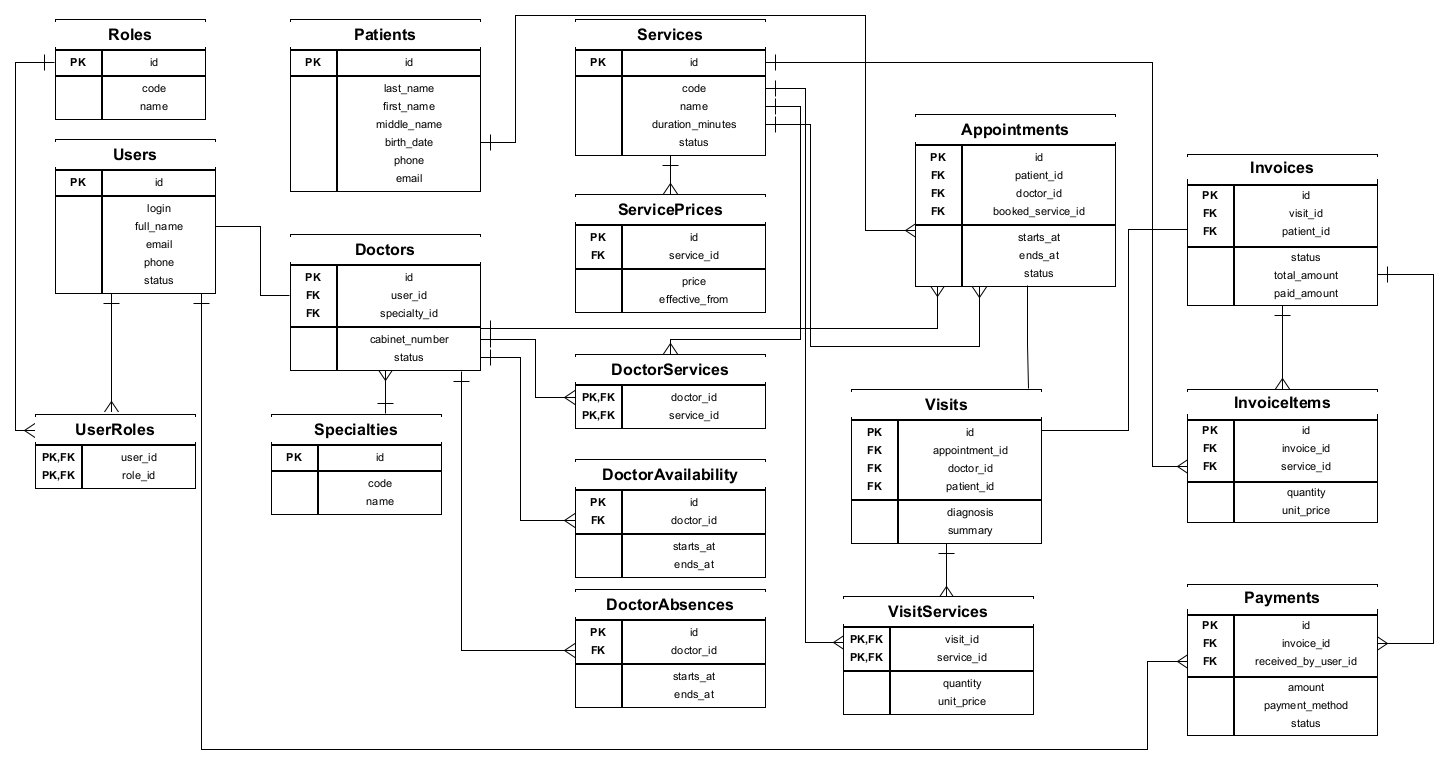
\includegraphics[width=\textwidth,height=1.1\textheight,keepaspectratio]{../diagrams/svg/Db_diagr.png}
    \caption{Схема проектируемой базы данных медицинской клиники}
    \label{fig:db-diagram}
\end{figure}

\clearpage
\section{Описание сущностей}

В разработанной базе данных сущности сгруппированы по функциональным схемам PostgreSQL. Такое разбиение соответствует фактической реализации проекта и позволяет разделить подсистемы безопасности, справочников, медицинских данных, расписания и расчетов.

\subsection{Подсистема безопасности}

Таблица \texttt{security.roles} хранит перечень ролей базы данных прикладного уровня. Для каждой роли задаются уникальные атрибуты \texttt{code} и \texttt{name}, позволяющие однозначно идентифицировать назначение роли.

Таблица \texttt{security.users} описывает учетные записи пользователей системы. В ней хранятся логин, хэш пароля, полное имя, контактные данные и статус учетной записи. Данная таблица используется для учетных записей прикладных пользователей системы: пациента, администратора и врача, а также для фиксации автора операций записи, отмены и приема оплаты.

Таблица \texttt{user\_roles} задает связь <<пользователь -- роль>>. Через нее одному пользователю могут быть назначены несколько ролей.

\subsection{Справочные сущности}

Таблица \texttt{catalog.specialties} содержит справочник врачебных специальностей. Записи этой таблицы используются при описании врачей и при группировке расписания и отчетов по профилю врача.

Таблица \texttt{catalog.services} описывает медицинские услуги, доступные в клинике. Для услуги хранятся код, наименование, описание, нормативная длительность приема и статус доступности. Именно эта сущность используется как при планировании записи, так и при формировании фактически оказанных услуг.

Таблица \texttt{catalog.service\_prices} хранит историю стоимости услуг. Для каждой цены задаются дата начала действия, дата окончания действия и стоимость в валюте \texttt{RUB}. Таким образом обеспечивается возможность расчета стоимости услуг с учетом периода действия прайс-листа.

\subsection{Медицинские сущности}

Таблица \texttt{medical.patients} хранит сведения о пациентах: фамилию, имя, отчество, дату рождения, контактные данные, номер страхового полиса и статус записи о пациенте. Эта таблица используется при записи на прием, ведении истории обращений и формировании счетов.

Таблица \texttt{medical.doctors} описывает врачей клиники. Каждая запись связана с учетной записью пользователя и со специальностью, а также содержит номер кабинета и статус врача. Связь с таблицей \texttt{security.users} имеет характер один-к-одному, что позволяет разделить сведения о сотруднике и сведения о доступе в систему.

Таблица \texttt{doctor\_services} реализует связь многие-ко-многим между врачами и услугами. Она определяет, какие услуги конкретный врач имеет право выполнять.

Таблица \texttt{medical.visits} фиксирует факт проведенного приема. Она связана с конкретной записью на прием, а также содержит ссылки на врача и пациента, диагноз и краткое описание результата приема.

Таблица \texttt{medical.visit\_services} содержит перечень услуг, фактически оказанных в рамках приема. Для каждой позиции сохраняются количество, цена за единицу и итоговая стоимость строки, что позволяет далее автоматически формировать счет.

\subsection{Сущности расписания и записи}

Таблица \texttt{scheduling.doctor\_availability} описывает интервалы доступности врача для записи. Для каждого интервала задаются начало и окончание периода, длительность слота и признак активности расписания.

Таблица \texttt{scheduling.doctor\_absences} хранит интервалы отсутствия врача с указанием причины. Эти данные используются при контроле доступности времени записи и при проверке возможности проведения приема.

Таблица \texttt{scheduling.appointments} описывает записи пациентов на прием. Она связывает пациента, врача и планируемую услугу, хранит время начала и окончания приема, статус записи, служебное примечание, причину отмены, а также ссылки на пользователей, создавших или отменивших запись. Данная таблица является центральной сущностью операционного контура базы данных.

\subsection{Финансовые сущности}

Таблица \texttt{billing.invoices} хранит счета, сформированные по результатам проведенного приема. Каждый счет связан с одним приемом и пациентом, а также содержит итоговую сумму, сумму оплаты и текущий статус расчета.

Таблица \texttt{billing.invoice\_items} содержит позиции счета. Каждая позиция связывает счет с конкретной услугой и хранит количество, цену и стоимость строки. Содержимое данной таблицы формируется на основе таблицы \texttt{medical.visit\_services}.

Таблица \texttt{billing.payments} хранит сведения об оплатах по счетам. Для каждой оплаты фиксируются сумма, способ оплаты, статус, внешний идентификатор операции и пользователь, зарегистрировавший оплату.

Таким образом, основная цепочка предметной области в реализованной базе данных выглядит следующим образом: пациент или администратор формирует запись пациента к врачу на услугу, проведенный прием порождает запись о визите и перечень оказанных услуг, после чего на их основе формируется счет и регистрируются оплаты.

\section{Ограничения целостности}

\subsection{Домены и перечислимые типы}

В схеме используются домены PostgreSQL \texttt{security.email\_address} и \texttt{security.phone\_number}. Они задают единые правила проверки e-mail и телефона и позволяют централизованно использовать один формат в таблицах пользователей и пациентов.

Для описания состояний сущностей применяются перечислимые типы PostgreSQL. Это исключает появление произвольных строковых значений и фиксирует допустимые переходы между состояниями. Модель статусов приведена в таблице~\ref{tab:status-model}.

\begin{table}[H]
    \centering
    \caption{Модель статусов и перечислимых типов PostgreSQL}
    \label{tab:status-model}
    \footnotesize
    \renewcommand{\arraystretch}{1.1}
    \setlength{\tabcolsep}{4pt}
    \begin{tabularx}{\textwidth}{|>{\raggedright\arraybackslash}p{2.85cm}|>{\raggedright\arraybackslash}p{4.15cm}|>{\raggedright\arraybackslash}X|}
        \hline
        Сущность & Тип PostgreSQL & Допустимые значения \tabularnewline
        \hline
        Пользователь & \begin{tabular}[t]{@{}l@{}}{\scriptsize\texttt{security.}}\tabularnewline{\scriptsize\texttt{user\_status}}\end{tabular} & active, inactive, archived \tabularnewline
        \hline
        Пациент & \begin{tabular}[t]{@{}l@{}}{\scriptsize\texttt{medical.}}\tabularnewline{\scriptsize\texttt{patient\_status}}\end{tabular} & active, inactive, archived \tabularnewline
        \hline
        Врач & \begin{tabular}[t]{@{}l@{}}{\scriptsize\texttt{medical.}}\tabularnewline{\scriptsize\texttt{doctor\_status}}\end{tabular} & active, inactive, archived \tabularnewline
        \hline
        Услуга & \begin{tabular}[t]{@{}l@{}}{\scriptsize\texttt{catalog.}}\tabularnewline{\scriptsize\texttt{service\_status}}\end{tabular} & active, inactive, archived \tabularnewline
        \hline
        Запись на прием & \begin{tabular}[t]{@{}l@{}}{\scriptsize\texttt{scheduling.}}\tabularnewline{\scriptsize\texttt{appointment\_status}}\end{tabular} & \begin{tabular}[t]{@{}l@{}}booked, cancelled,\tabularnewline completed\end{tabular} \tabularnewline
        \hline
        Счет & \begin{tabular}[t]{@{}l@{}}{\scriptsize\texttt{billing.}}\tabularnewline{\scriptsize\texttt{invoice\_status}}\end{tabular} & \begin{tabular}[t]{@{}l@{}}issued, partially\_paid,\tabularnewline paid, cancelled\end{tabular} \tabularnewline
        \hline
        Оплата & \begin{tabular}[t]{@{}l@{}}{\scriptsize\texttt{billing.}}\tabularnewline{\scriptsize\texttt{payment\_status}}\end{tabular} & completed, cancelled \tabularnewline
        \hline
    \end{tabularx}
\end{table}
\normalsize

\subsection{Ключи и связи многие-ко-многим}

Во всех основных таблицах в качестве первичных ключей используются значения типа \texttt{UUID}. Такой подход позволяет формировать идентификаторы независимо от конкретного клиента. Он также не раскрывает информацию о количестве записей.

Ссылочная целостность обеспечивается внешними ключами. Связи многие-ко-многим реализованы тремя промежуточными таблицами:
\begin{itemize}
    \item \texttt{doctor\_services} --- связь <<врач -- услуга>>;
    \item \texttt{visit\_services} --- связь <<прием -- оказанная услуга>>;
    \item \texttt{user\_roles} --- связь <<пользователь -- роль>>.
\end{itemize}

\subsection{Ограничения времени и запрет конфликтов}

Для таблиц истории цен, доступности врача, отсутствий врача и записей на прием используются диапазоны типа \texttt{TSTZRANGE}. Это позволяет единообразно хранить временные интервалы и применять к ним ограничения пересечения.

Для предотвращения двойной записи у одного врача используется ограничение \texttt{EXCLUDE}. Оно запрещает пересечение интервалов времени у активных записей и тем самым обеспечивает бесконфликтную работу в многопользовательском режиме.

\subsection{Доказательство 3НФ}

Спроектированная база данных находится в третьей нормальной форме по следующим причинам:
\begin{enumerate}
    \item все таблицы имеют первичный ключ, а их атрибуты являются атомарными;
    \item в таблицах со составным ключом, таких как \texttt{doctor\_services}, \texttt{visit\_services} и \texttt{user\_roles}, неключевые атрибуты не зависят от части ключа;
    \item транзитивные зависимости устранены выделением самостоятельных сущностей для ролей, специальностей, истории цен, оказанных услуг, счетов и оплат.
\end{enumerate}

Следовательно, каждый неключевой атрибут зависит только от ключа, от полного ключа и ни от чего, кроме ключа, что и соответствует требованиям 3НФ.

\section{Процедуры, функции и триггеры}

На уровне базы данных реализованы процедуры делового регламента и вспомогательные функции. Они обеспечивают контроль прав, выбор актуальной цены, пересчет счета и автоматическое обновление служебных полей.

\subsection{Вспомогательные функции}

Функция \texttt{set\_updated\_at} используется триггерами для автоматического обновления поля \texttt{updated\_at} перед изменением записи. Схема функции приведена на рисунке~\ref{fig:yed-set-updated-at}.

\begin{figure}[H]
    \centering
    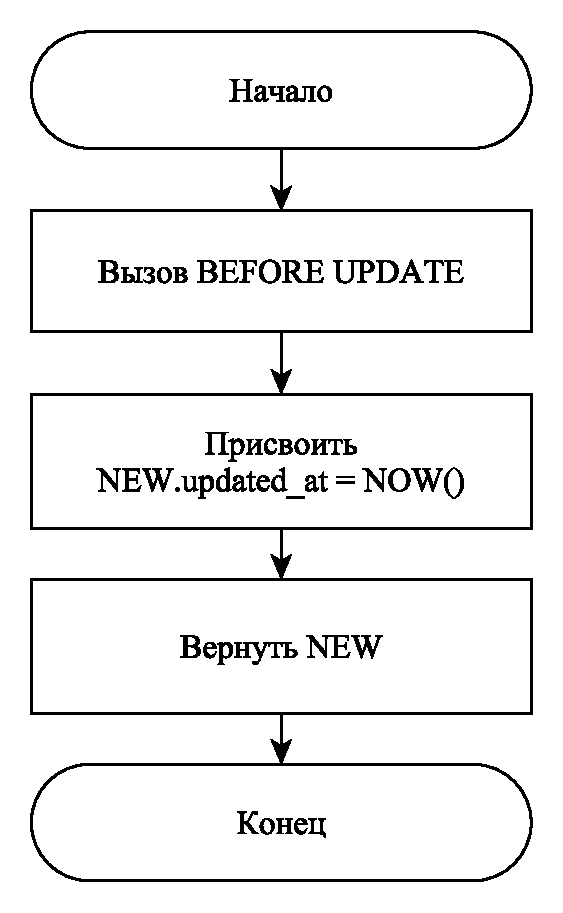
\includegraphics[width=0.40\textwidth]{figures/yed_set_updated_at.pdf}
    \caption{Схема функции \texttt{set\_updated\_at}}
    \label{fig:yed-set-updated-at}
\end{figure}

Функция \texttt{has\_role} проверяет наличие прикладной роли у пользователя. Схема функции приведена на рисунке~\ref{fig:yed-has-role}.

\begin{figure}[H]
    \centering
    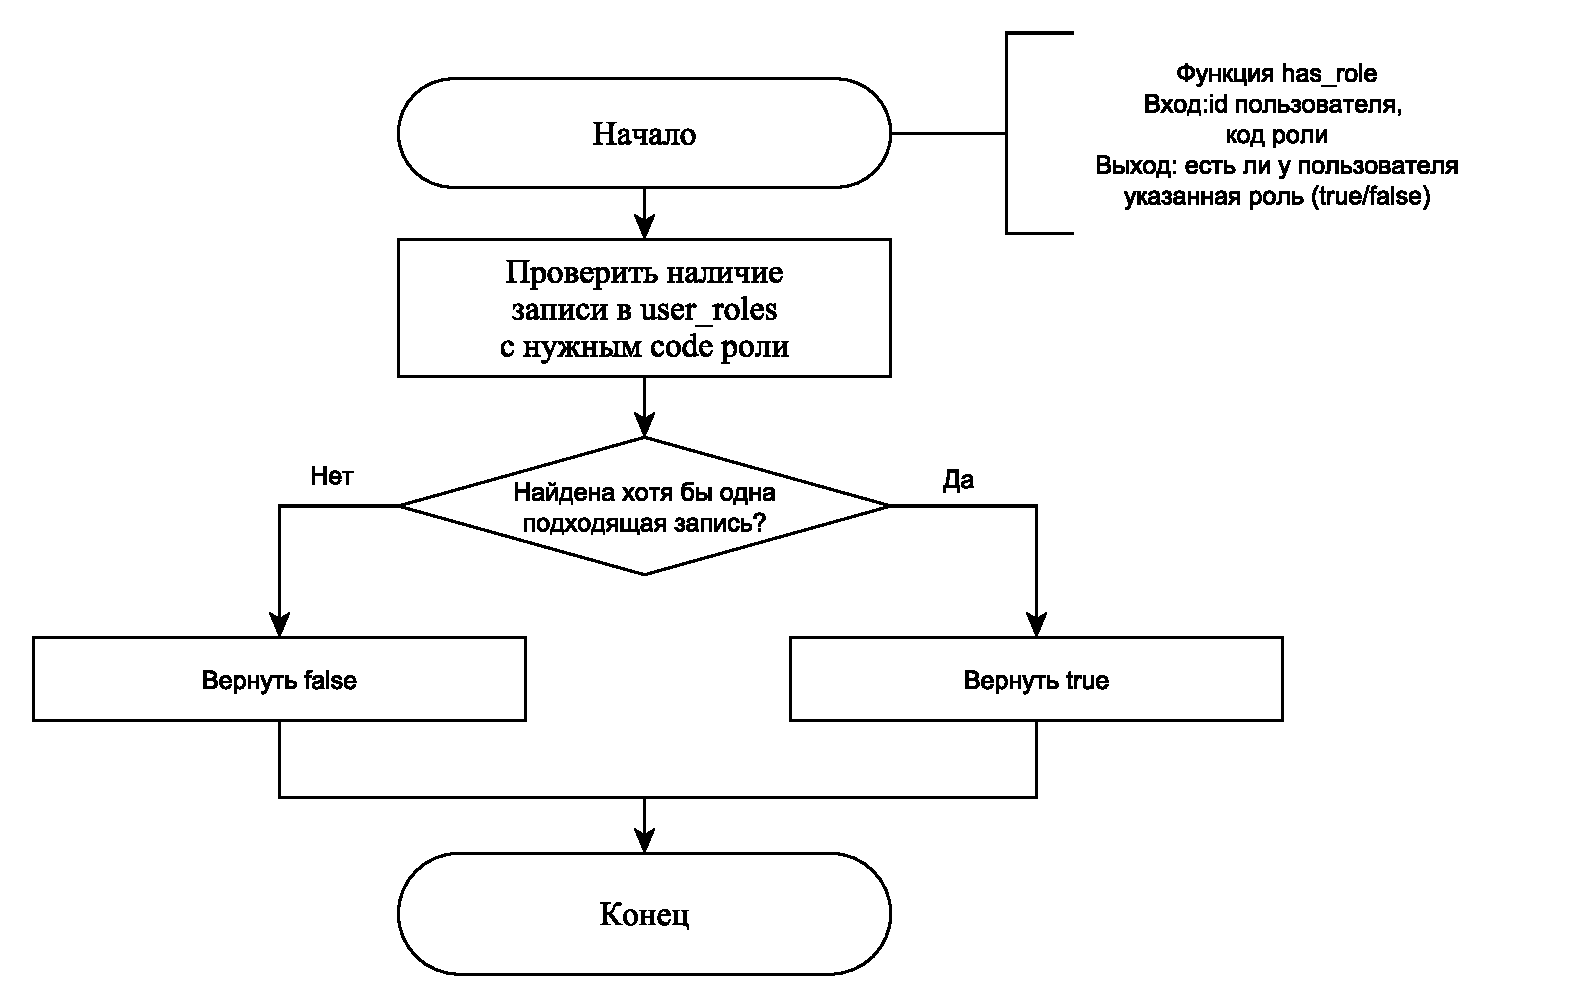
\includegraphics[width=0.74\textwidth]{figures/yed_has_role.pdf}
    \caption{Схема функции \texttt{has\_role}}
    \label{fig:yed-has-role}
\end{figure}

Функция \texttt{get\_service\_price} выбирает актуальную цену услуги на заданный момент времени. Схема функции приведена на рисунке~\ref{fig:yed-get-service-price}.

\begin{figure}[H]
    \centering
    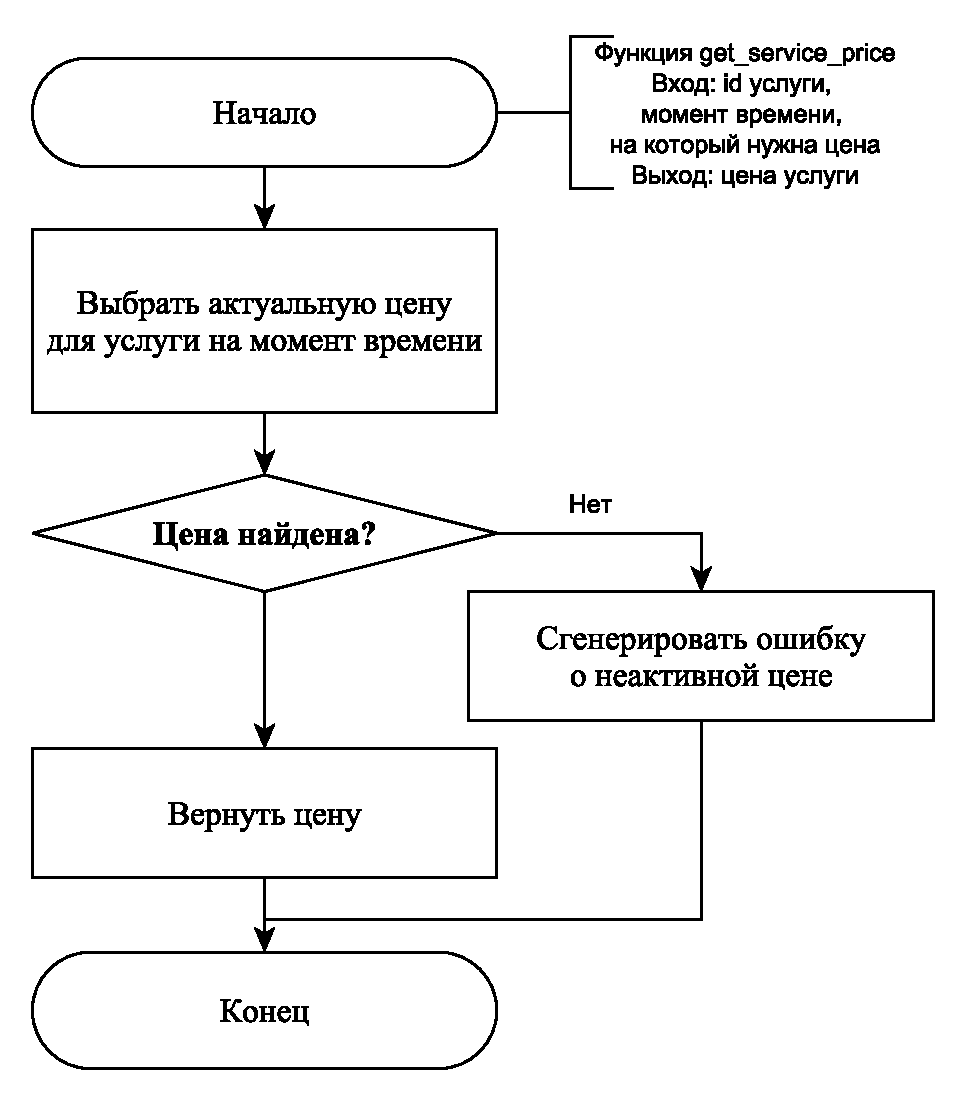
\includegraphics[width=0.6\textwidth]{figures/yed_get_service_price.pdf}
    \caption{Схема функции \texttt{get\_service\_price}}
    \label{fig:yed-get-service-price}
\end{figure}

\subsection{Процедуры делового регламента}

Схема процедуры записи на прием приведена на рисунке~\ref{fig:design-book-appointment}.

Функция \texttt{book\_appointment} проверяет время начала приема, активность пациента и врача, закрепление услуги за врачом и активность самой услуги. Затем вычисляется время окончания приема, проверяются интервал доступности врача и отсутствие записи о его отсутствии. Конфликт по времени дополнительно предотвращается ограничением \texttt{EXCLUDE} при вставке записи.

\begin{figure}[H]
    \centering
    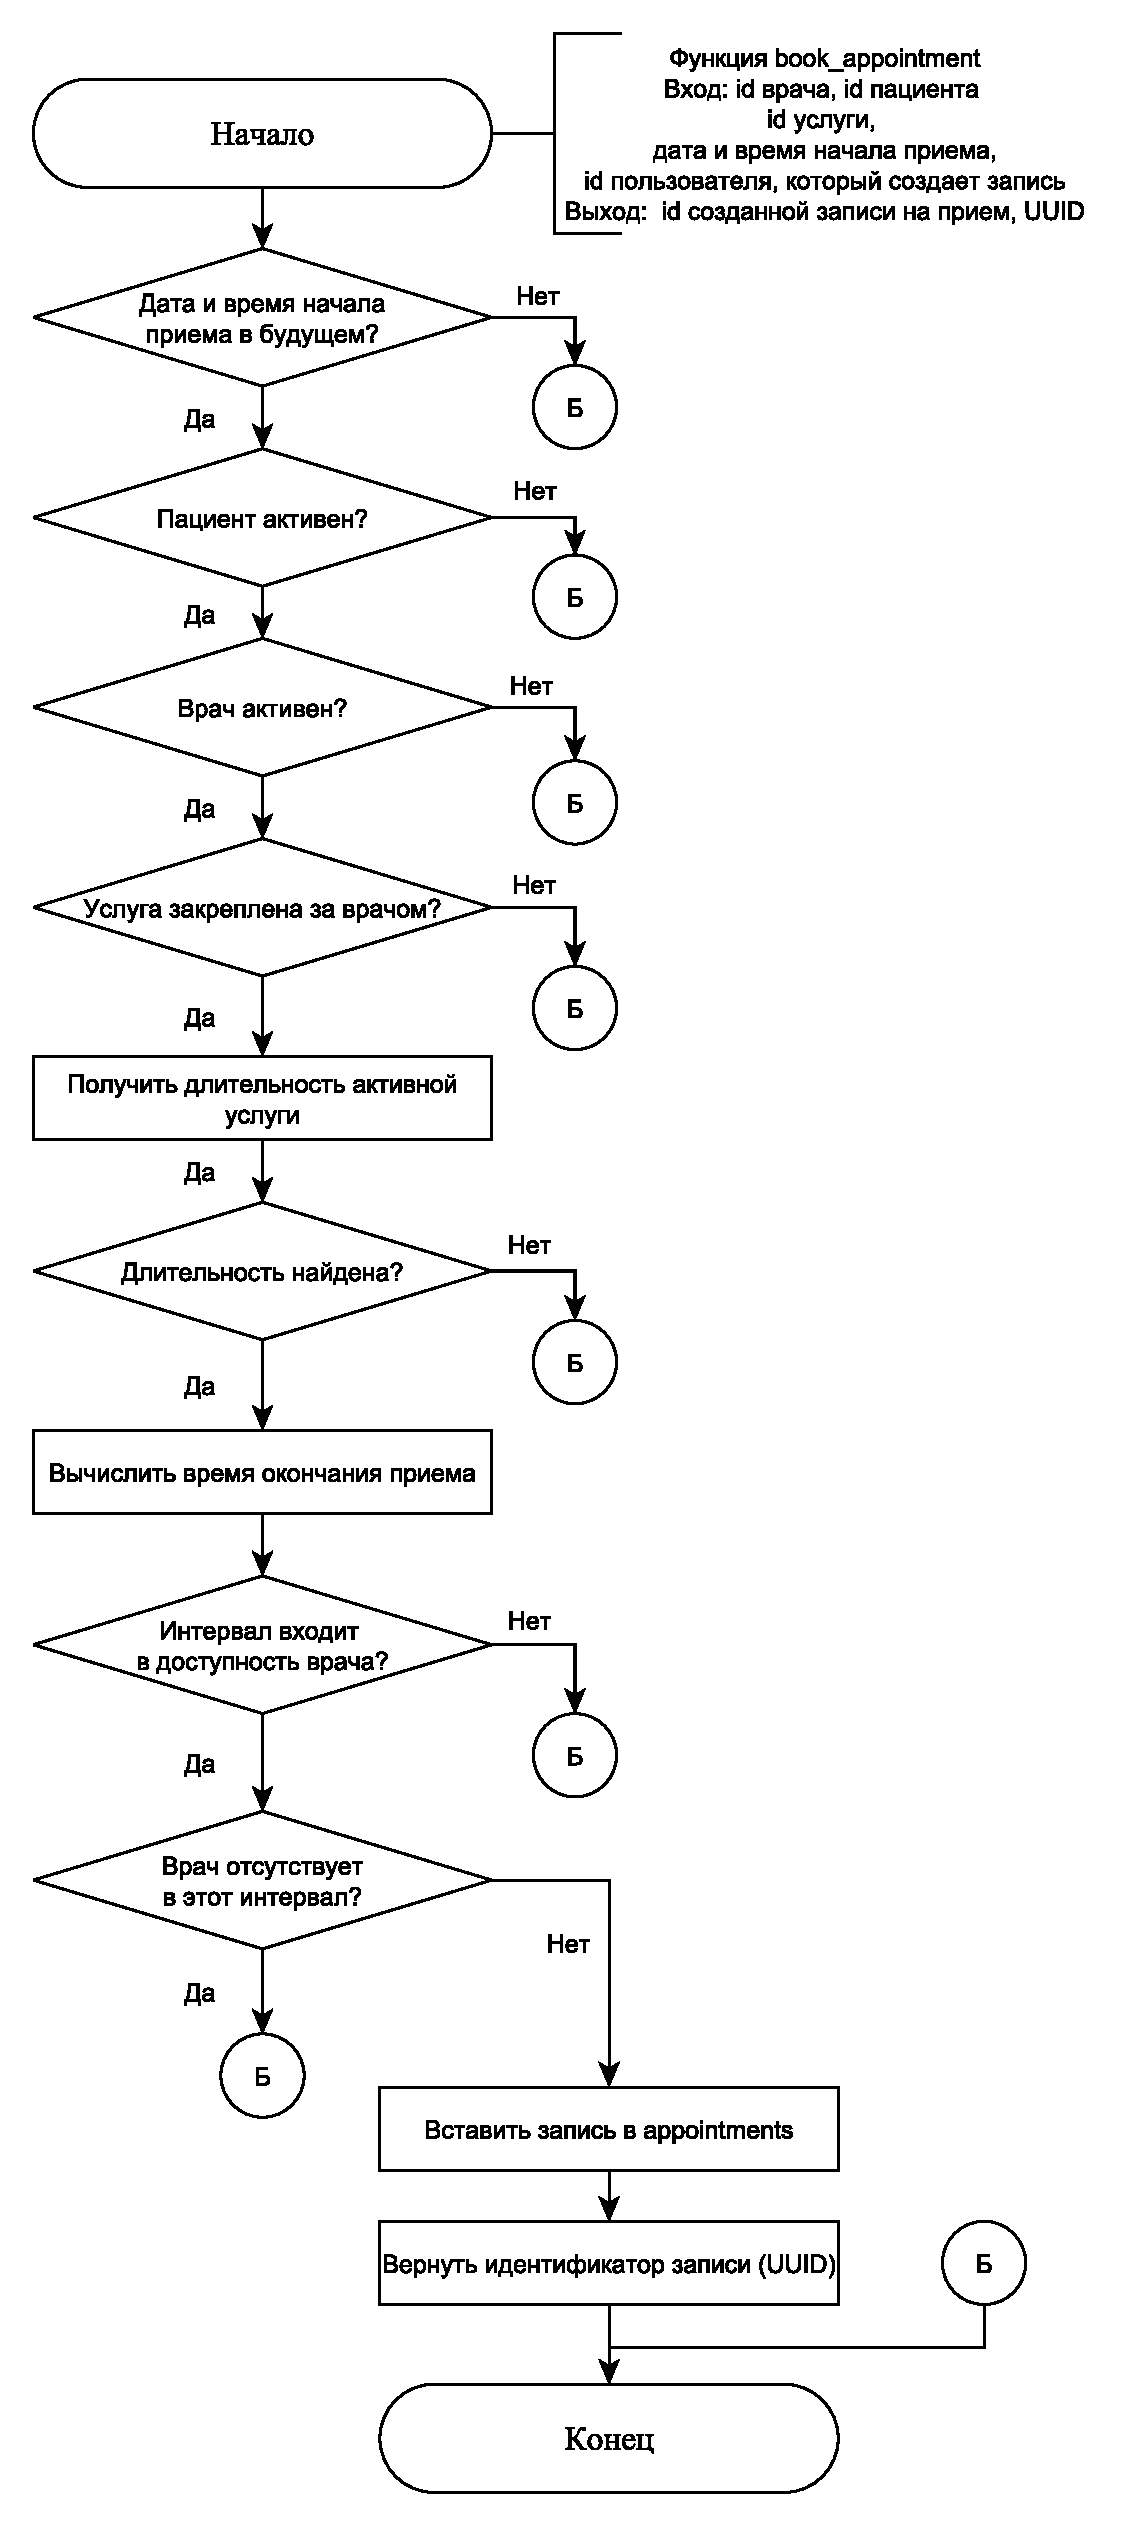
\includegraphics[height=0.90\textheight,keepaspectratio]{figures/yed_book_appointment.pdf}
    \caption{Схема функции \texttt{book\_appointment}}
    \label{fig:design-book-appointment}
\end{figure}

\newpage

Схема отмены записи приведена на рисунке~\ref{fig:design-cancel-appointment}.

Функция \texttt{cancel\_appointment} блокирует строку записи и проверяет ее состояние. Для пациента дополнительно действует правило отмены не позднее чем за 24 часа до приема, тогда как администратор может выполнить отмену без этого ограничения.

\begin{figure}[H]
    \centering
    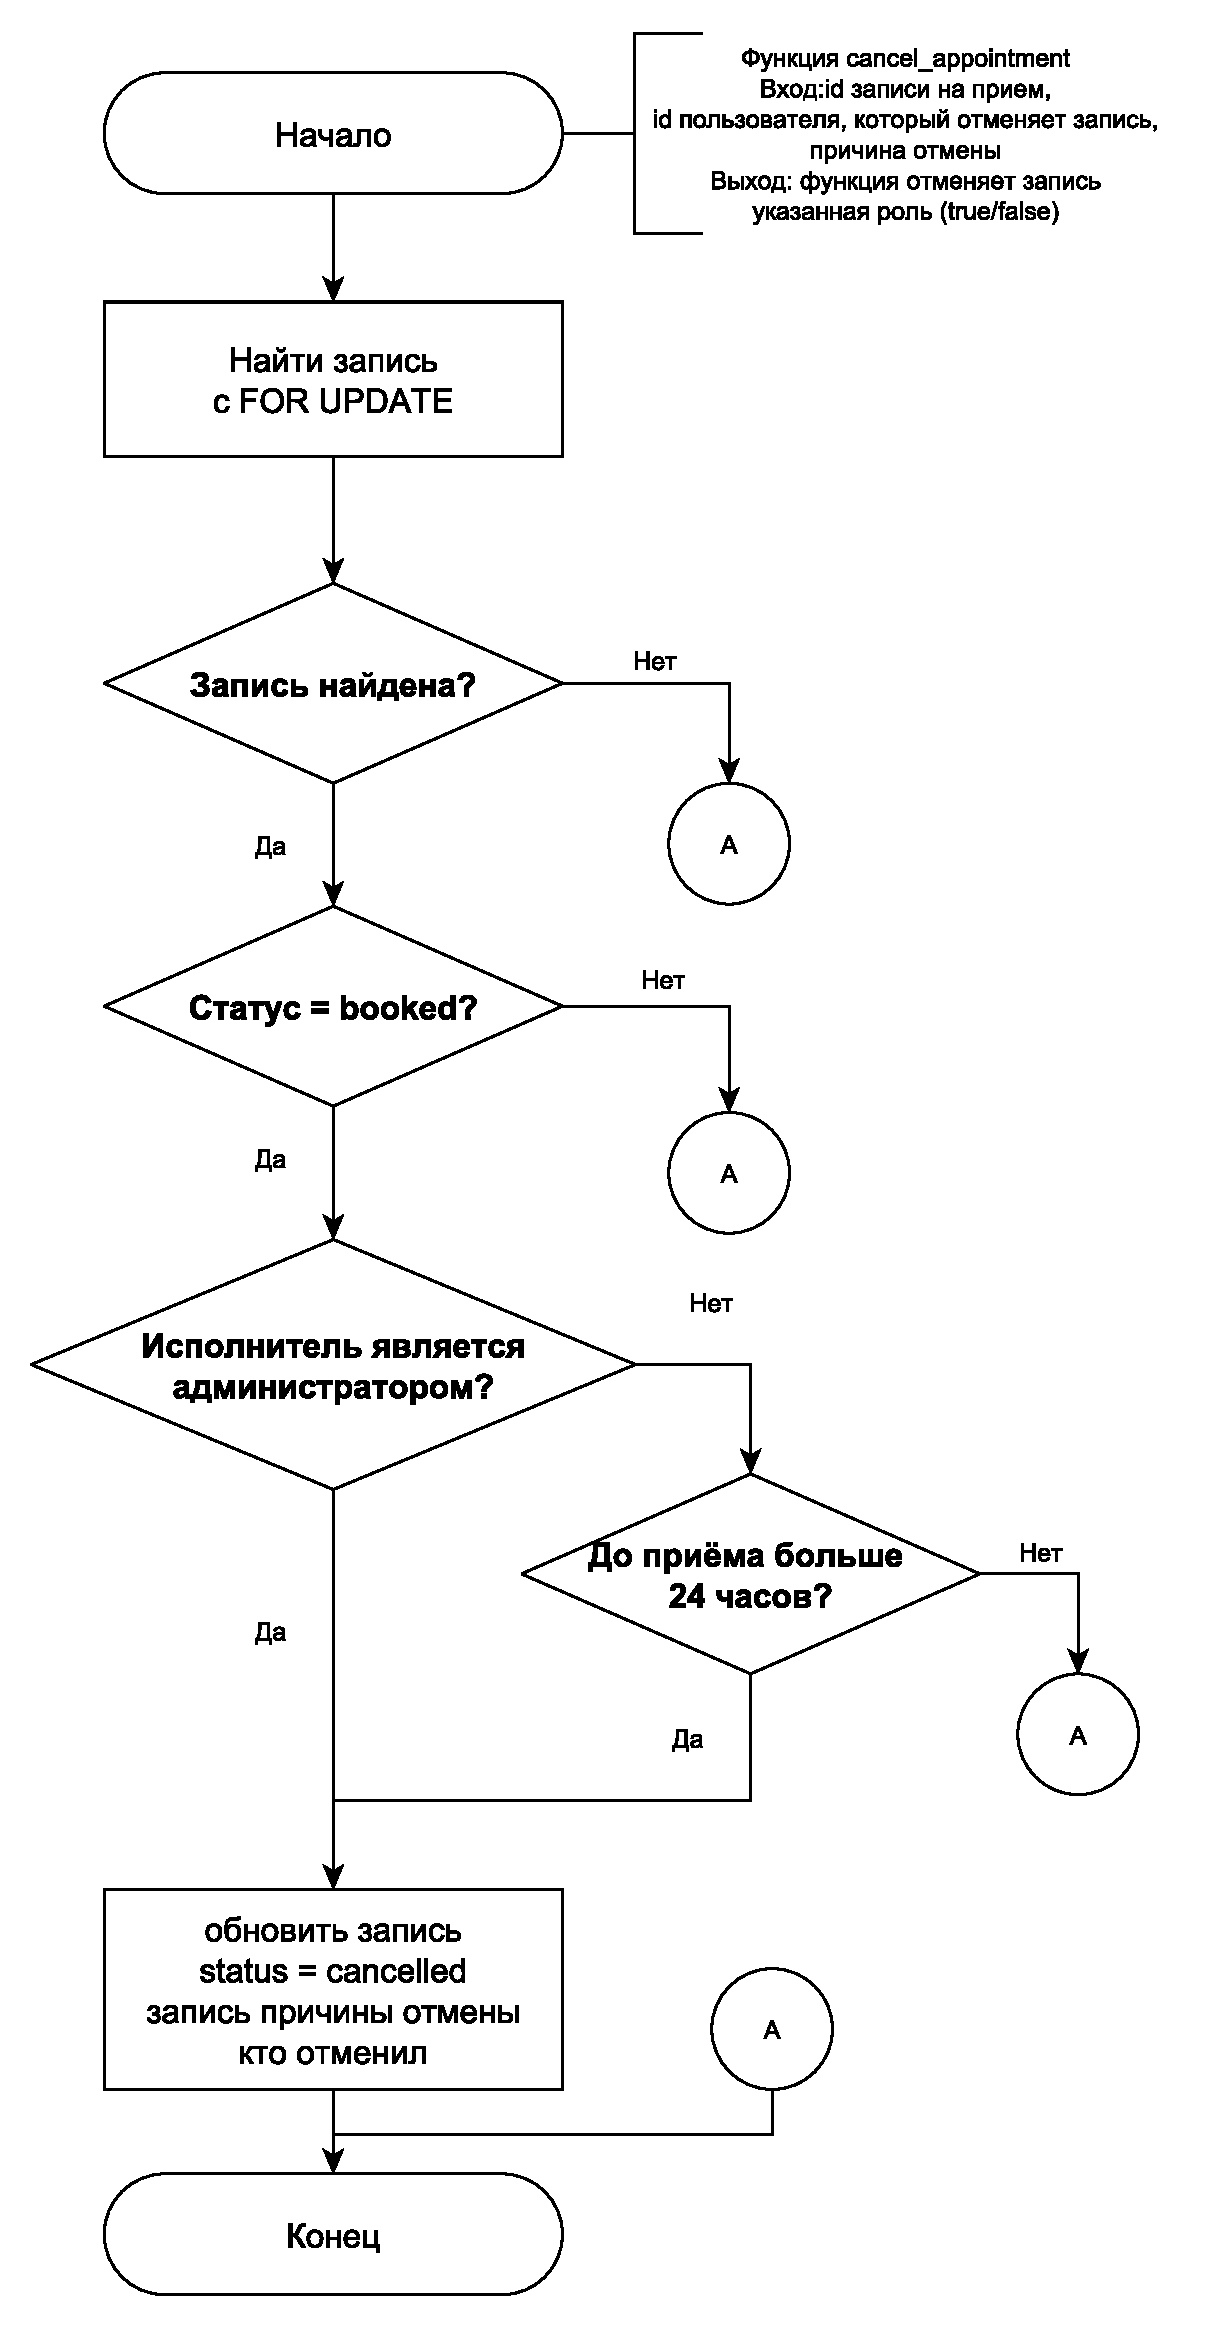
\includegraphics[width=0.70\textwidth]{figures/yed_cancel_appointment.pdf}
    \caption{Схема функции \texttt{cancel\_appointment}}
    \label{fig:design-cancel-appointment}
\end{figure}

\newpage

Схема функции проведения приема приведена на рисунке~\ref{fig:design-complete-visit}.

Функция \texttt{complete\_visit} создает запись о визите и фиксирует оказанные услуги. Если список оказанных услуг пуст, в \texttt{visit\_services} заносится забронированная услуга; иначе обрабатывается переданный список услуг. Затем формируются счет и строки счета, запись на прием переводится в состояние \texttt{completed}, после чего вызывается \texttt{refresh\_invoice\_state}.

\begin{figure}[H]
    \centering
    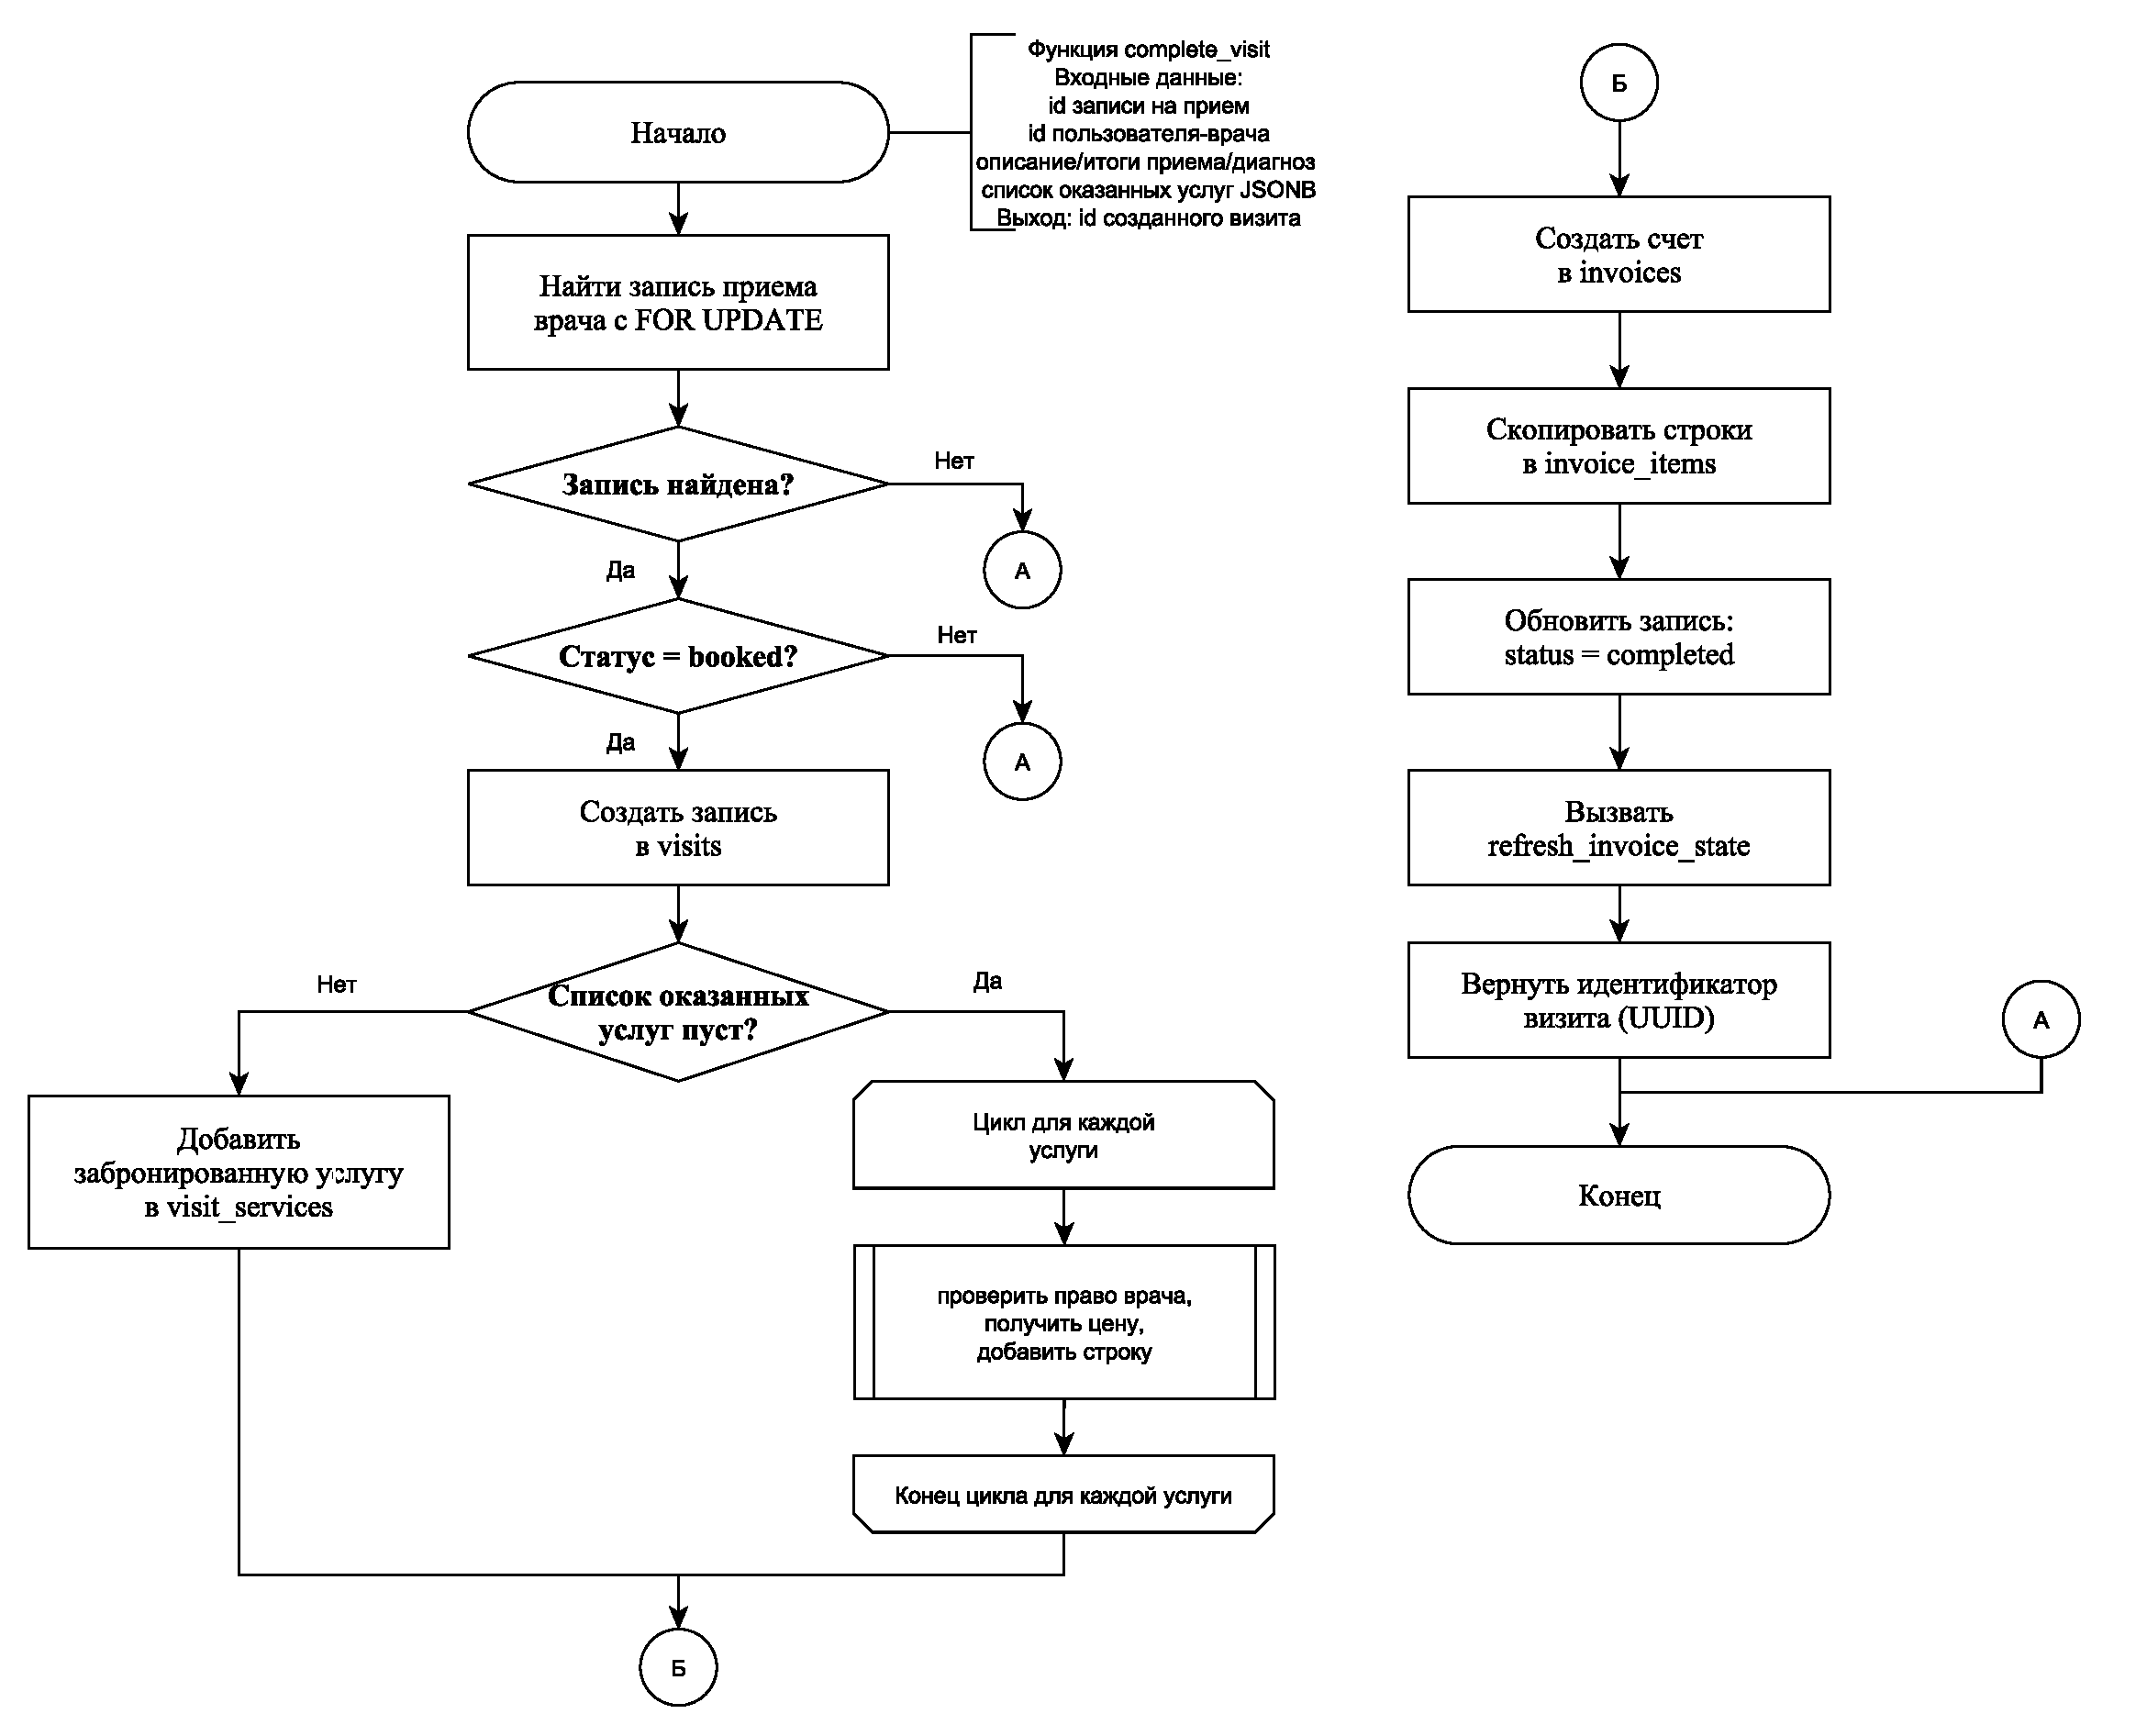
\includegraphics[width=0.8\textwidth]{figures/yed_complete_visit.pdf}
    \caption{Схема функции \texttt{complete\_visit}}
    \label{fig:design-complete-visit}
\end{figure}

\newpage

Схема регистрации оплаты приведена на рисунке~\ref{fig:design-register-payment}.

Функция \texttt{register\_payment} создает запись об оплате. Затем инициируется пересчет состояния счета.

\begin{figure}[H]
    \centering
    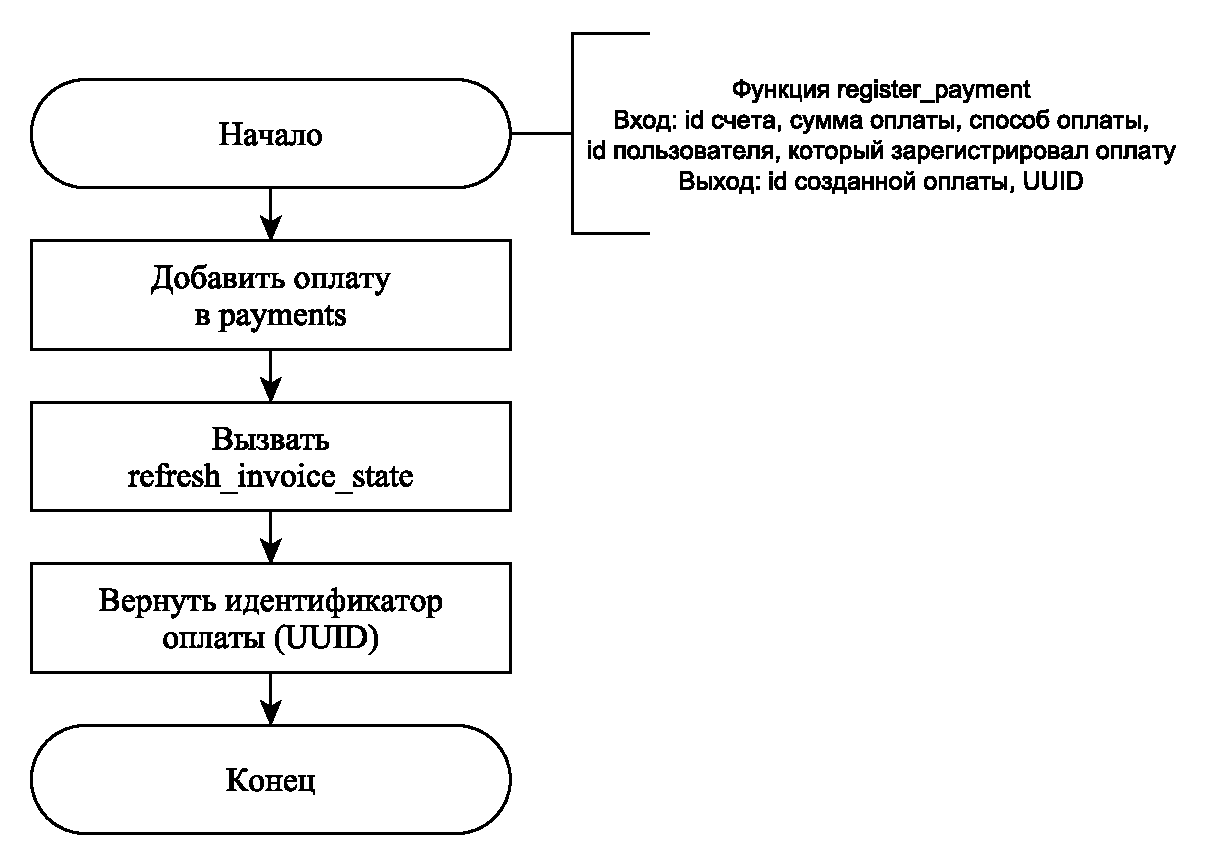
\includegraphics[width=0.55\textwidth]{figures/yed_register_payment.pdf}
    \caption{Схема функции \texttt{register\_payment}}
    \label{fig:design-register-payment}
\end{figure}

\subsection{Функции пересчета счета и триггеры}

Схема функции \texttt{refresh\_invoice\_state} приведена на рисунке~\ref{fig:design-refresh-invoice-state}.

Функция \texttt{refresh\_invoice\_state} вычисляет итоговую сумму счета, сумму проведенных оплат и итоговый статус расчета.

\begin{figure}[H]
    \centering
    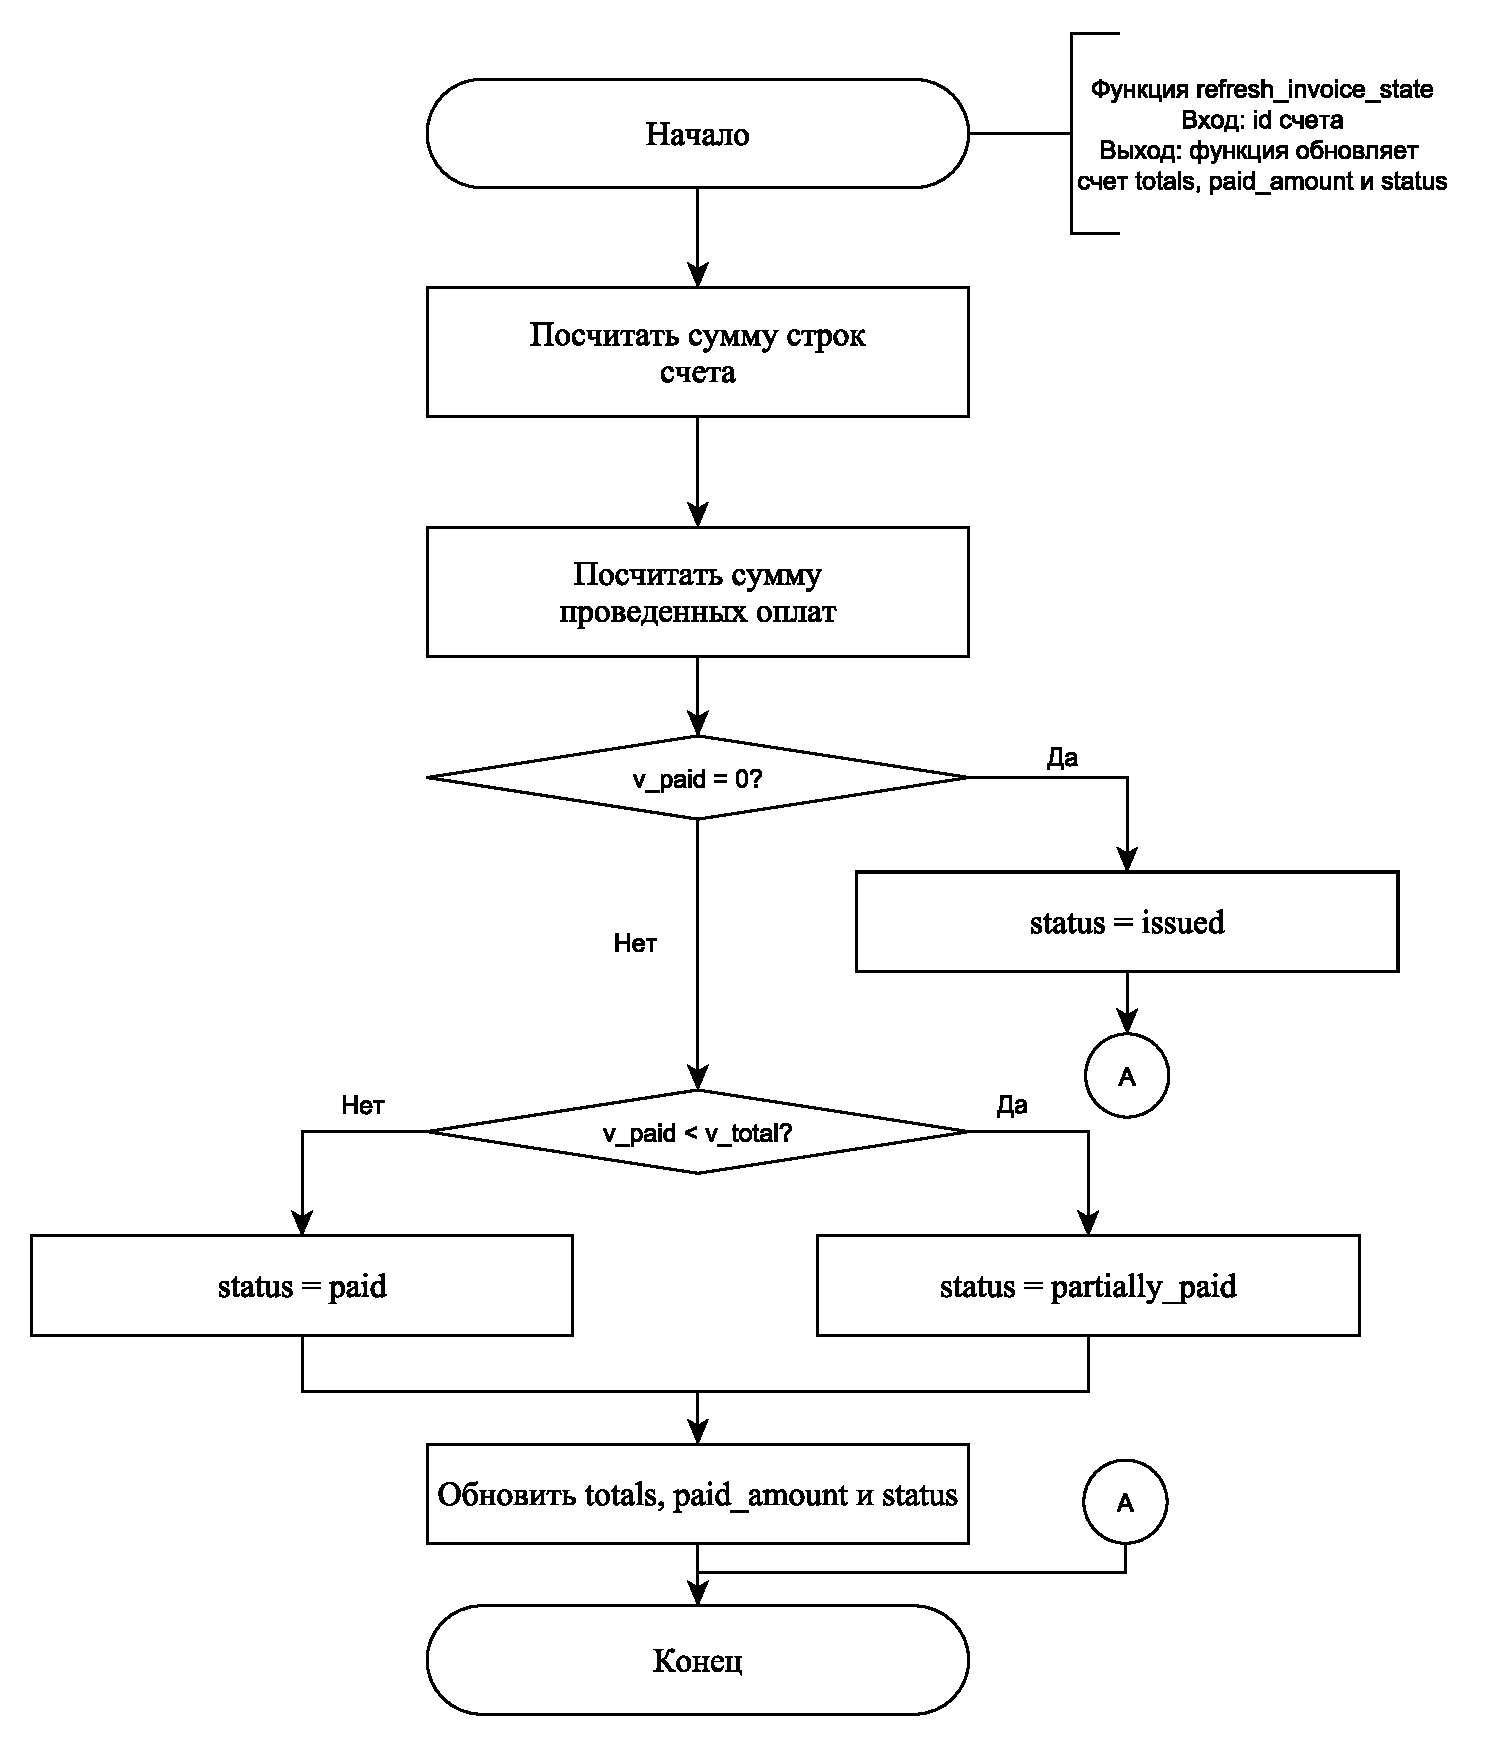
\includegraphics[width=0.74\textwidth]{figures/yed_refresh_invoice_state.pdf}
    \caption{Схема функции \texttt{refresh\_invoice\_state}}
    \label{fig:design-refresh-invoice-state}
\end{figure}

Схема триггеров пересчета счета приведена на рисунке~\ref{fig:design-refresh-invoice-triggers}.

Триггеры \texttt{trg\_\allowbreak{}invoice\_\allowbreak{}items\_\allowbreak{}refresh\_\allowbreak{}invoice} и \texttt{trg\_\allowbreak{}payments\_\allowbreak{}refresh\_\allowbreak{}invoice} срабатывают после изменения строк счета или оплат, определяют идентификатор счета и вызывают функцию \texttt{refresh\_\allowbreak{}invoice\_\allowbreak{}state}.

\begin{figure}[H]
    \centering
    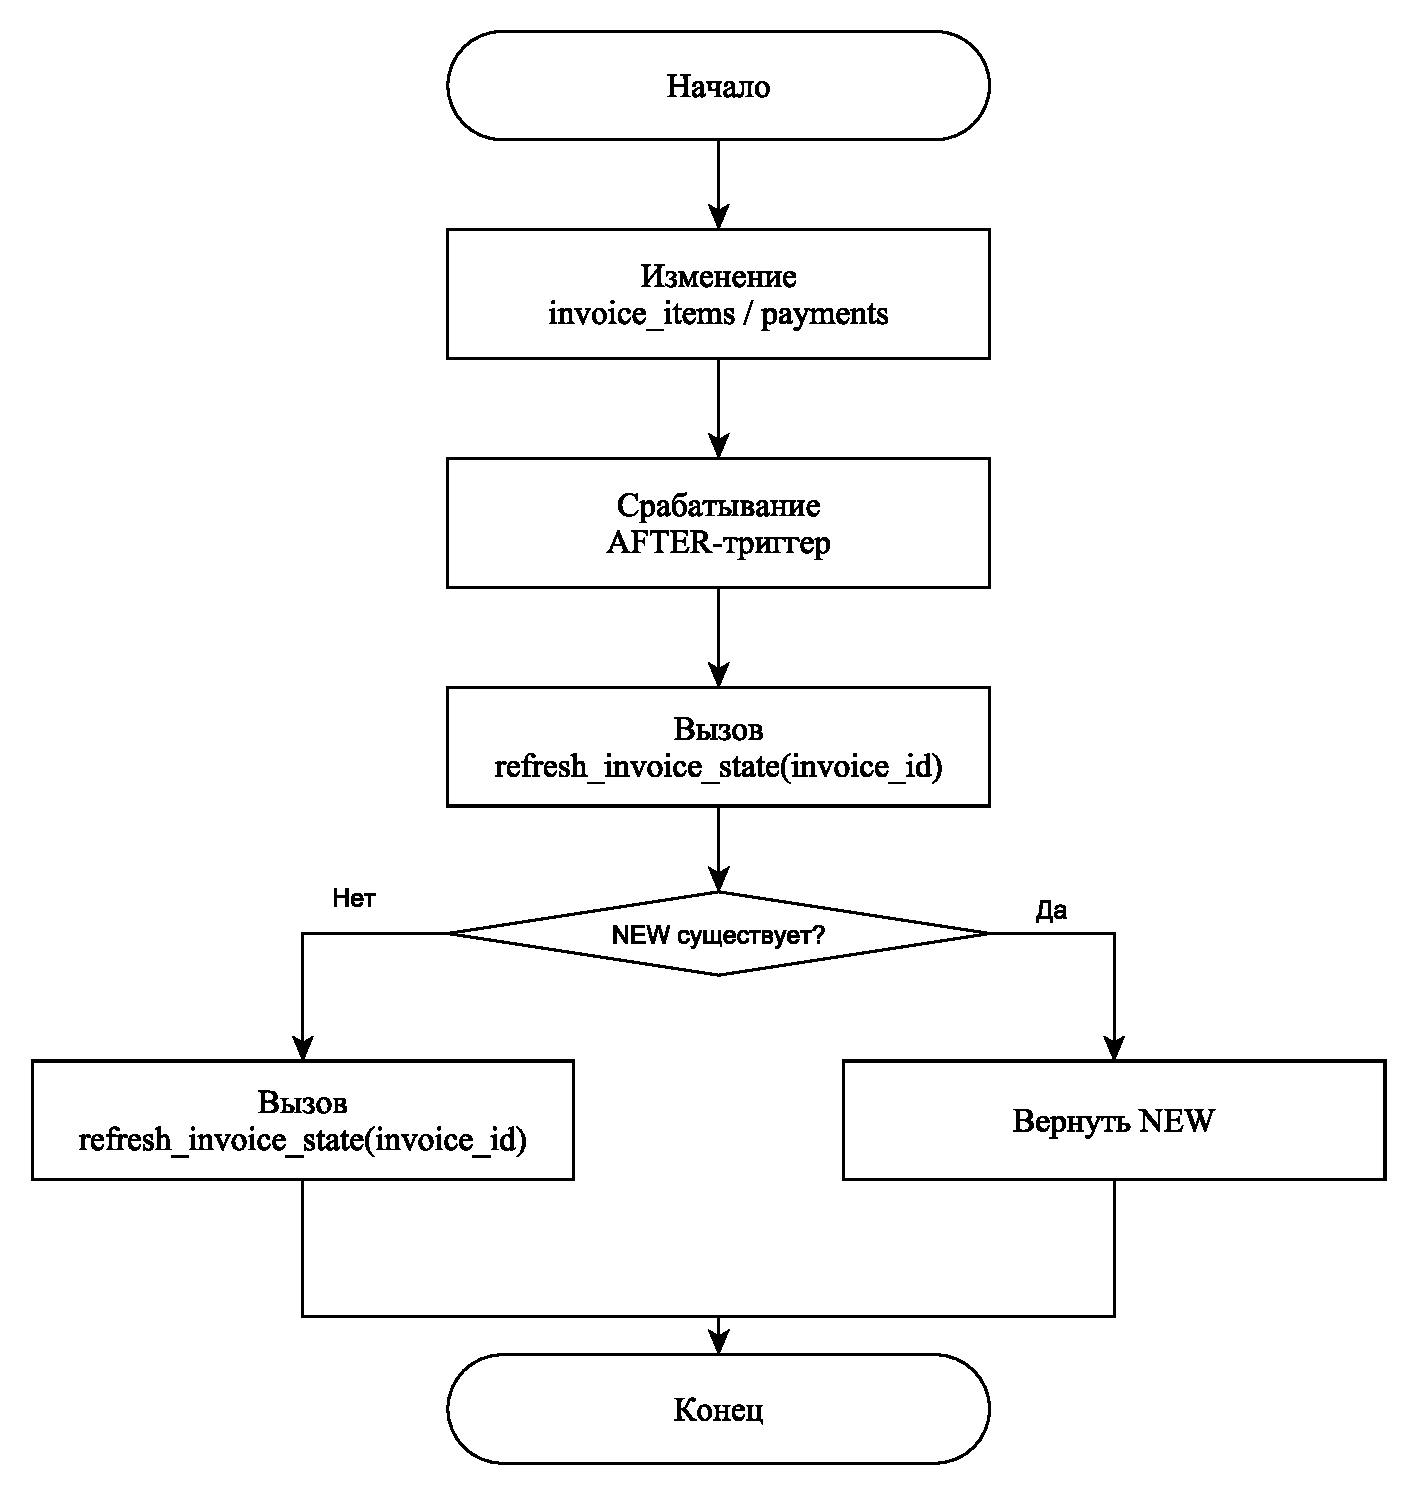
\includegraphics[width=0.68\textwidth]{figures/yed_refresh_invoice_triggers.pdf}
    \caption{Схема триггеров пересчета счета}
    \label{fig:design-refresh-invoice-triggers}
\end{figure}



Перечень триггеров базы данных приведен в таблице~\ref{tab:db-triggers}.

\begin{table}[H]
    \centering
    \caption{Триггеры базы данных}
    \label{tab:db-triggers}
    \footnotesize
    \renewcommand{\arraystretch}{1.12}
    \setlength{\tabcolsep}{4pt}
    \begin{tabularx}{\textwidth}{|>{\raggedright\arraybackslash}p{4.10cm}|>{\raggedright\arraybackslash}p{4.75cm}|>{\raggedright\arraybackslash}X|}
        \hline
        Имя триггера & Таблица и событие & Назначение \tabularnewline
        \hline
        \parbox[t]{4.10cm}{\raggedright{\scriptsize\texttt{trg\_\*\_}}\newline {\scriptsize\texttt{updated\_at}}} &
        \parbox[t]{4.75cm}{\raggedright{\scriptsize\texttt{users, patients,}}\newline {\scriptsize\texttt{doctors, services,}}\newline {\scriptsize\texttt{appointments, visits,}}\newline {\scriptsize\texttt{invoices,}}\newline {\scriptsize\texttt{doctor\_availability,}}\newline {\scriptsize\texttt{doctor\_absences;}}\newline событие {\scriptsize\texttt{BEFORE UPDATE}}} &
        Автоматическое обновление поля \texttt{updated\_at} \tabularnewline
        \hline
        \parbox[t]{4.10cm}{\raggedright{\scriptsize\texttt{trg\_invoice\_items\_}}\newline {\scriptsize\texttt{refresh\_invoice}}} &
        \parbox[t]{4.75cm}{\raggedright{\scriptsize\texttt{billing.invoice\_items;}}\newline событие {\scriptsize\texttt{AFTER INSERT,}}\newline {\scriptsize\texttt{UPDATE, DELETE}}} &
        Пересчет суммы и статуса счета \tabularnewline
        \hline
        \parbox[t]{4.10cm}{\raggedright{\scriptsize\texttt{trg\_payments\_}}\newline {\scriptsize\texttt{refresh\_invoice}}} &
        \parbox[t]{4.75cm}{\raggedright{\scriptsize\texttt{billing.payments;}}\newline событие {\scriptsize\texttt{AFTER INSERT,}}\newline {\scriptsize\texttt{UPDATE, DELETE}}} &
        Пересчет суммы оплат и статуса счета \tabularnewline
        \hline
    \end{tabularx}
\end{table}

\section{Ролевая модель базы данных}

Следует различать прикладные роли системы и роли базы данных.

Прикладные роли описывают, кто работает в интерфейсе системы, например пациент, администратор или врач. Ролевая модель базы данных описывает роли PostgreSQL и выданные им привилегии на объекты схемы.

В конструкторском разделе требуется именно ролевая модель на уровне базы данных.

В реализованной схеме используются три роли PostgreSQL:
\begin{itemize}
    \item \texttt{clinic\_owner};
    \item \texttt{clinic\_api};
    \item \texttt{clinic\_reporting}.
\end{itemize}
Их назначение приведено в таблице~\ref{tab:db-role-model}.

\begin{table}[H]
    \centering
    \caption{Ролевая модель базы данных}
    \label{tab:db-role-model}
    \footnotesize
    \renewcommand{\arraystretch}{1.1}
    \setlength{\tabcolsep}{4pt}
    \begin{tabularx}{\textwidth}{|>{\raggedright\arraybackslash}p{3.0cm}|>{\raggedright\arraybackslash}p{3.3cm}|>{\raggedright\arraybackslash}X|}
        \hline
        Роль PostgreSQL & Назначение & Предоставляемые права \tabularnewline
        \hline
        \texttt{clinic\_owner} & \begin{tabular}[t]{@{}l@{}}Владелец схемы\tabularnewline базы данных\end{tabular} & \begin{tabular}[t]{@{}l@{}}Создание и изменение схем, таблиц,\tabularnewline индексов, процедур, триггеров и ролей\end{tabular} \tabularnewline
        \hline
        \texttt{clinic\_api} & \begin{tabular}[t]{@{}l@{}}Роль backend-\tabularnewline приложения\end{tabular} & \begin{tabular}[t]{@{}l@{}}USAGE на схемы;\tabularnewline SELECT, INSERT, UPDATE, DELETE\tabularnewline для рабочих таблиц;\tabularnewline EXECUTE для процедур и функций\end{tabular} \tabularnewline
        \hline
        \begin{tabular}[t]{@{}l@{}}\texttt{clinic\_}\tabularnewline\texttt{reporting}\end{tabular} & \begin{tabular}[t]{@{}l@{}}Роль отчетов\tabularnewline и аналитики\end{tabular} & \begin{tabular}[t]{@{}l@{}}Доступ только на чтение к данным,\tabularnewline необходимым для формирования отчетов\end{tabular} \tabularnewline
        \hline
    \end{tabularx}
\end{table}
\normalsize

Прикладные роли пользователей не дублируются отдельными SQL-ролями. Они контролируются на уровне приложения и работают через backend, использующий роль \texttt{clinic\_api}.

Таким образом, разграничение доступа на уровне интерфейса и на уровне СУБД остаются разделенными и не смешиваются в одной модели.

\section{Транзакционная стратегия и требования к кэшированию}

Критические операции --- запись на прием, отмена записи, проведение приема и регистрация оплаты --- выполняются в транзакционном контексте.

Контроль согласованности сосредоточен в PostgreSQL. Он обеспечивается сочетанием транзакций, ограничений целостности, диапазонных типов и исключающих ограничений.

Для ускорения чтения в Redis кэшируются два объекта:
\begin{itemize}
    \item текущий прайс-лист услуг по ключу \texttt{clinic:catalog:pricelist} с временем жизни 600 секунд;
    \item расписание врача по ключу вида \texttt{clinic:schedule:doctor:...} с временем жизни 600 секунд.
\end{itemize}

Кэш расписания инвалидируется после записи на прием, отмены записи и проведения приема. Кэш прайс-листа обновляется при повторном чтении после истечения времени жизни записи.

\section{Вывод}

В конструкторском разделе спроектирована структура базы данных медицинской клиники, доказано соответствие 3НФ, описаны ограничения целостности, процедуры, функции, триггеры, ролевая модель базы данных и правила кэширования. Полученная схема соответствует требованиям проекта и обеспечивает основу для дальнейшей реализации приложения.

\clearpage
